Chương này trình bày quá trình hiện thực hoá và đánh giá hệ thống GraphRAG đã được thiết kế ở Chương 3. Nội dung được tổ chức thành ba phần: (i) cài đặt hệ thống, (ii) thực nghiệm định lượng và (iii) triển khai kèm kiểm nghiệm với người dùng.

\section{Cài đặt và phát triển hệ thống}
\label{sec:system_setup}

Hệ thống được phát triển trên máy cá nhân chạy Windows và đóng gói để triển khai trên Google Cloud Run phục vụ giai đoạn kiểm nghiệm với người dùng (Mục~\ref{sec:user_deployment}). Knowledge Graph Chèo được dựng trên Neo4j, gồm bảy vở chèo cổ, 38 nhân vật, 41 diễn viên, 15 trích đoạn và 27 phiên bản biểu diễn; pipeline GraphRAG với cả ba chiến lược tạo sinh Pre/Mid/Post-Generation được cài đặt đầy đủ và có thể chuyển đổi qua cấu hình. Mô hình ngôn ngữ lớn được sử dụng qua API để đảm bảo tính \textit{LLM-agnostic}; một mô hình duy nhất được chọn làm mô hình chính cho toàn bộ thực nghiệm với tham số sinh cố định (temperature bằng 0, top-p bằng 1) để đảm bảo khả năng tái lập.

Ngoài GraphRAG, hai hệ thống khác được triển khai làm tham chiếu cho các thí nghiệm so sánh ở Mục~\ref{sec:experiments}. Hệ thống thứ nhất là \textbf{RAG truyền thống}. Trong đó, tài liệu mô tả nghệ thuật Chèo được chia thành các đoạn văn bản có độ dài cố định, nhúng véc-tơ bằng một mô hình embedding và lưu trong vector store. Khi nhận câu hỏi, hệ thống tính độ tương đồng cosine giữa véc-tơ câu hỏi và toàn bộ véc-tơ đoạn văn, lấy một số đoạn gần nhất làm ngữ cảnh trước khi gửi tới mô hình ngôn ngữ. Hệ thống thứ hai là \textbf{LLM-only}. Trong hệ thống này, câu hỏi được gửi trực tiếp tới mô hình ngôn ngữ kèm một prompt hệ thống ngắn xác định miền nghệ thuật Chèo, không có cơ chế truy xuất. Hệ thống này có tác dụng tách biệt đóng góp của cơ chế truy xuất so với tri thức nội tại của các LLMs hiện nay.

Cả ba hệ thống sử dụng cùng một mô hình ngôn ngữ và cùng tham số tạo sinh để chênh lệch kết quả chỉ phản ánh khác biệt về nguồn tri thức và cơ chế truy xuất. Prompt của RAG truyền thống và LLM-only được thiết kế đơn giản, chỉ yêu cầu trả lời bằng tiếng Việt dựa trên ngữ cảnh được cung cấp nếu có, không áp dụng các ràng buộc cấu trúc như trong ba chiến lược tạo sinh của GraphRAG. Cách thiết kế này giữ cho các thực nghiệm phản ánh đúng đặc trưng gốc, tránh việc kết quả được cải thiện một cách nhân tạo bởi các kỹ thuật prompting nâng cao.

\section{Thực nghiệm}
\label{sec:experiments}

\subsection{Mục tiêu và câu hỏi nghiên cứu}

Thực nghiệm nhằm đánh giá một cách hệ thống hiệu quả của kiến trúc GraphRAG đề xuất đối với việc khai thác tri thức có cấu trúc trong miền nghệ thuật Chèo, đồng thời phân tích đóng góp của từng thành phần trong kiến trúc. Bốn câu hỏi nghiên cứu được xác lập:

\begin{enumerate}
  \item Mức độ truy xuất trong Knowledge Graph ảnh hưởng như thế nào đến hiệu năng tổng thể?
  \item Định dạng biểu diễn ngữ cảnh tác động ra sao đến khả năng suy luận của mô hình ngôn ngữ?
  \item Chiến lược tạo sinh có cải thiện tính trung thực và độ chính xác của câu trả lời hay không?
  \item So với các hệ thông RAG truyền thống và LLM-only, GraphRAG mang lại lợi ích gì trong miền tri thức có cấu trúc quan hệ phức tạp?
\end{enumerate}

% Cần chỉnh sửa thêm
\subsection{Kiểm chứng tính hợp lệ của CheoBench v2}
\label{sec:benchmark_validity}

Tính hợp lệ của bộ dữ liệu được đánh giá trên bốn chiều theo khung Messick~\cite{messick1995validity}: bao phủ nội dung, cấu trúc độ khó, khả năng phân biệt hệ thống và nhất quán của hệ độ đo. Số liệu được tính từ bộ câu hỏi và từ kết quả 100 câu ở Mục~\ref{sec:experiments}.

Về bao phủ nội dung, 100 câu hỏi liệt kê 225 thực thể trong trường \\ \texttt{related\_entities}; đối chiếu với Knowledge Graph, bộ câu hỏi phủ 7/7 vở chèo, 25/34 nhân vật, 23/41 diễn viên và 8/15 trích đoạn (Bảng~\ref{tab:coverage_entity}). Toàn bộ 225 thực thể đều khớp với định danh trong KG, không câu nào yêu cầu tri thức ngoài phạm vi hệ thống. Coverage ở lớp vở đạt 100\%; các lớp con dao động từ 53\% đến 73\%, tập trung vào các thực thể trung tâm theo thực hành của BEIR~\cite{thakur2021beir}. 100 câu hỏi được phân vào 10 subcategory khác nhau, trải trên nhiều dạng truy vấn.

\begin{table}[h]
\centering
\caption{Mức độ bao phủ của CheoBench v2 trên Knowledge Graph Chèo.}
\label{tab:coverage_entity}
\begin{tabular}{lrrr}
\hline
\textbf{Loại thực thể} & \textbf{Đã phủ} & \textbf{Tổng} & \textbf{Tỷ lệ} \\
\hline
Vở chèo       &  7 &  7 & 100.0\% \\
Nhân vật      & 25 & 34 &  73.5\% \\
Diễn viên     & 23 & 41 &  56.1\% \\
Trích đoạn    &  8 & 15 &  53.3\% \\
\hline
\end{tabular}
\end{table}

Về cấu trúc độ khó, Edge et al.~\cite{edge2024graphrag} dự đoán khoảng cách GraphRAG--RAG giảm dần từ truy vấn Local (ánh xạ tên riêng) đến truy vấn Global (tổng hợp toàn cục). Bảng~\ref{tab:construct_validity} xác nhận xu hướng này trên 100 câu hỏi: khoảng cách giảm đơn điệu từ +0,309 (Local) qua +0,245 (Community) xuống +0,163 (Global). Số thực thể liên quan trung bình cũng phân tách ba nhóm ở mức 1,94 (Local), 2,50 (Community) và 2,33 (Global).

\begin{table}[h]
\centering
\caption{Khoảng cách hiệu năng GraphRAG--RAG theo nhóm truy vấn.}
\label{tab:construct_validity}
\begin{tabular}{lcccc}
\hline
\textbf{Nhóm} & \textbf{\#Ents TB} & \textbf{GraphRAG} & \textbf{RAG} & \textbf{Khoảng cách} \\
\hline
Local      & 1.94 & 0.862 & 0.553 & +0.309 \\
Community  & 2.50 & 0.861 & 0.616 & +0.245 \\
Global     & 2.33 & 0.782 & 0.619 & +0.163 \\
\hline
\end{tabular}
\end{table}

Về khả năng phân biệt hệ thống, trên 100 cặp (GraphRAG, RAG) không có cặp hoà điểm, 94 cặp GraphRAG đạt điểm cao hơn, $\Delta = S_{\text{GraphRAG}} - S_{\text{RAG}}$ có trung bình +0,240 và độ lệch chuẩn 0,193. Phân phối trải rộng với 72\% cặp có $|\Delta| \geq 0{,}10$ và 33\% cặp có $|\Delta| \geq 0{,}30$ (Bảng~\ref{tab:discrimination}), cho phép phân biệt hai hệ thống ở nhiều cấp độ thay vì ở hai cực.

\begin{table}[h]
\centering
\caption{Phân phối khoảng cách điểm tổng hợp $\Delta = S_{\text{GraphRAG}} - S_{\text{RAG}}$ trên 100 câu hỏi.}
\label{tab:discrimination}
\begin{tabular}{lrr}
\hline
\textbf{Chỉ số} & \textbf{Giá trị} & \textbf{Tỷ lệ} \\
\hline
Câu có GraphRAG $\geq$ RAG & 94/100 & 94.0\% \\
Câu hoà điểm ($|\Delta| < 10^{-6}$) &  0/100 &  0.0\% \\
Câu có $|\Delta| \geq 0.05$ & 84/100 & 84.0\% \\
Câu có $|\Delta| \geq 0.10$ & 72/100 & 72.0\% \\
Câu có $|\Delta| \geq 0.20$ & 50/100 & 50.0\% \\
Câu có $|\Delta| \geq 0.30$ & 33/100 & 33.0\% \\
\hline
Trung bình $\Delta$ & +0.240 & --- \\
Độ lệch chuẩn của $\Delta$ &  0.193 & --- \\
\hline
\end{tabular}
\end{table}

Về nhất quán của hệ độ đo, Cronbach's $\alpha$~\cite{cronbach1951alpha} tính trên điểm per-case của GraphRAG cho khối IR năm độ đo (MAP, NDCG@10, Precision, Recall, ContextEntitiesRecall) đạt 0,790, vượt ngưỡng 0,70~\cite{nunnally1978psychometric}; $\alpha$ toàn cục chín độ đo là 0,699 (Bảng~\ref{tab:consistency}). Hai khối Context và Generation có $\alpha$ gần 0, cho thấy các cặp độ đo trong mỗi khối đo các khía cạnh khác nhau (độ liên quan so với độ bao phủ; độ trung thực so với độ phù hợp). Tương quan Pearson bổ sung: $r(\text{MAP}, \text{NDCG@10}) = 0{,}98$, Faithfulness trực giao với các độ đo khác ($|r| \leq 0{,}06$), ContextEntitiesRecall tương quan yếu với mọi độ đo ($|r| \leq 0{,}14$). Bộ chín độ đo do đó vừa có khối nhất quán nội tại, vừa có các chiều bổ sung trực giao.

\begin{table}[h]
\centering
\caption{Cronbach's $\alpha$ của các khối độ đo trên 100 câu hỏi (hệ thống GraphRAG).}
\label{tab:consistency}
\begin{tabular}{lcc}
\hline
\textbf{Khối độ đo} & \textbf{Số độ đo} & \textbf{Cronbach's $\alpha$} \\
\hline
Toàn bộ                   & 9 & 0.699 \\
Khối IR xác định          & 5 & \textbf{0.790} \\
Khối Context (RAGAs)      & 2 & $-0.048$ \\
Khối Generation (RAGAs)   & 2 & $-0.063$ \\
\hline
\end{tabular}
\end{table}


\subsection{Độ đo đánh giá}

\subsubsection{Chất lượng truy xuất}

Chất lượng truy xuất được đánh giá bởi bốn độ đo IR truyền thống kết hợp với ba độ đo ngữ nghĩa theo RAGAs~\cite{es2023ragas}. Nhóm IR gồm:

\begin{itemize}
  \item \textbf{MAP}~\cite{manning2008ir} --- trung bình độ chính xác (average precision) trên toàn bộ truy vấn; trong bài toán này, MAP thưởng các cấu hình đưa nhiều thực thể đúng lên vị trí đầu của danh sách truy xuất, phản ánh chất lượng xếp hạng tổng thể.

  \item \textbf{NDCG@10}~\cite{jarvelin2002ndcg} --- đánh giá chất lượng xếp hạng ở mười vị trí đầu với phạt logarit theo vị trí; mức cắt $K = 10$ được chọn để phù hợp với kích thước ngữ cảnh điển hình mà pipeline đưa vào mô hình ngôn ngữ.

  \item \textbf{Precision} và \textbf{Recall} --- tỷ lệ chính xác và độ bao phủ của kết quả truy xuất so với tập thực thể liên quan $R$ theo ground truth, tính trên toàn bộ danh sách truy xuất $L$ sau khi loại trùng lặp:
    \begin{equation}
      \text{Precision} = \frac{|L \cap R|}{|L|}, \qquad \text{Recall} = \frac{|L \cap R|}{|R|}.
    \end{equation}
\end{itemize}

Ba độ đo ngữ nghĩa theo RAGAs \cite{es2023ragas} bổ sung cho các độ đo IR ở khía cạnh ngữ nghĩa và đều nằm trong thang $[0, 1]$. \textbf{Context Precision} và \textbf{Context Recall} được mô hình ngôn ngữ chấm điểm từ cặp (câu hỏi, ngữ cảnh) và (ground truth, ngữ cảnh) để ước lượng tỷ lệ thông tin liên quan và mức độ bao phủ tri thức cần thiết. \textbf{Context Entities Recall} được tính trực tiếp: gọi $E$ là tập các thực thể bắt buộc theo ground truth, độ đo là tỷ lệ thực thể trong $E$ xuất hiện trong ngữ cảnh được truy xuất:

\begin{equation}
\text{Context Entities Recall} = \frac{|E \cap \text{context}|}{|E|}.
\end{equation}

Điểm truy xuất tổng hợp được tính theo công thức:

\begin{equation}
\begin{aligned}
S_{\text{retrieval}} =\;& 0.20 \cdot \text{MAP}
  + 0.15 \cdot \text{NDCG@10} \\
& + 0.10 \cdot \text{Precision}
  + 0.10 \cdot \text{Recall} \\
& + 0.20 \cdot \text{Context Precision}
  + 0.15 \cdot \text{Context Recall} \\
& + 0.10 \cdot \text{Context Entities Recall}.
\end{aligned}
\end{equation}

Trước hết, khối IR được đánh trọng số 0,55 - cao hơn khối RAGAs (0,45), do các độ đo IR có thể tính toán trực tiếp và tái lập chính xác, trong khi RAGAs phụ thuộc vào phán đoán của mô hình ngôn ngữ (LLM-judge) và có sự biến động giữa các lần chạy. Trong khối IR, MAP giữ trọng số cao nhất (0,20) do bao quát toàn bộ chất lượng xếp hạng trên mọi vị trí, NDCG@10 đứng thứ hai (0,15) do chỉ nhạy với mười vị trí đầu, còn Precision và Recall mỗi độ đo chỉ phản ánh một khía cạnh riêng - độ chính xác và độ bao phủ - nên được cân bằng ở 0,10.Trong khối RAGAs, Context Precision được ưu tiên cao nhất (0,20) vì ngữ cảnh chứa thông tin không liên quan dễ dẫn mô hình ngôn ngữ sai hướng và ảnh hưởng trực tiếp đến chất lượng câu trả lời, trong khi Context Recall (0,15) và Context Entities Recall (0,10) cùng đo độ bao phủ nhưng ở các phạm vi khác nhau, với Entities Recall hẹp hơn nên nhận trọng số thấp hơn.

Cơ chế tổng hợp xử lý trường hợp độ đo không khả dụng bằng tái chuẩn hoá. Khi một độ đo RAGAs trả về giá trị vô hiệu do lỗi tạm thời của mô hình, độ đo đó được loại khỏi công thức và các trọng số còn lại được chuẩn hoá lại về tổng 1. Điểm truy xuất do đó luôn được tính trên tập độ đo khả dụng cho từng câu hỏi, tránh việc lỗi kỹ thuật đơn lẻ làm giảm kết quả đánh giá.

\subsubsection{Chất lượng tạo sinh}

Chất lượng tạo sinh được đánh giá qua hai độ đo RAGAs~\cite{es2023ragas}, cả hai đều thuộc loại \textbf{LLM-as-judge} - mô hình ngôn ngữ đóng vai trò bên chấm điểm và trả về giá trị trong thang $[0, 1]$. \textbf{Faithfulness} đo tỷ lệ nội dung câu trả lời thực sự được ngữ cảnh truy xuất hỗ trợ, được thiết kế để phát hiện hallucination --- hiện tượng mô hình ngôn ngữ đưa ra thông tin không có trong ngữ cảnh. Giá trị của độ đo được tính qua hai bước, mỗi bước là một lần gọi mô hình ngôn ngữ:

\begin{enumerate}
  \item \textit{Tách mệnh đề.} Mô hình được yêu cầu liệt kê các khẳng định đơn lẻ trong câu trả lời, mỗi khẳng định trên một dòng. Gọi tập các mệnh đề thu được là $C = \{c_1, \ldots, c_n\}$. Ví dụ, câu trả lời ``Thị Kính là vợ của Thiện Sỹ và bị Sùng Bà vu oan'' được tách thành hai mệnh đề độc lập ``Thị Kính là vợ của Thiện Sỹ'' và ``Thị Kính bị Sùng Bà vu oan''.

  \item \textit{Kiểm chứng từng mệnh đề.} Với mỗi $c_i \in C$, mô hình được đưa ngữ cảnh truy xuất cùng với mệnh đề và được hỏi mệnh đề đó có được hỗ trợ hay không. Mệnh đề chỉ được tính là ``được hỗ trợ'' khi mô hình trả lời ``có''; các trường hợp ``không'' hoặc mơ hồ đều được coi là không hỗ trợ.
\end{enumerate}

Giá trị Faithfulness cuối cùng là tỷ lệ mệnh đề được hỗ trợ trên tổng số mệnh đề trích xuất được:

\begin{equation}
\text{Faithfulness} = \frac{|\{c \in C : \text{được ngữ cảnh hỗ trợ}\}|}{|C|}.
\end{equation}

\textbf{Answer Relevance} được mô hình ngôn ngữ ước lượng trực tiếp từ cặp (câu hỏi, câu trả lời), cho một điểm số liên tục phản ánh mức độ câu trả lời giải quyết đúng câu hỏi được đặt ra. Điểm tạo sinh tổng hợp hai độ đo với trọng số bằng nhau:

\begin{equation}
S_{\text{generation}} = 0.5 \cdot \text{Faithfulness} + 0.5 \cdot \text{Answer Relevance}.
\end{equation}

\subsubsection{Điểm tổng hợp}

Điểm tổng hợp $S_{\text{overall}}$ kết hợp $S_{\text{retrieval}}$ và $S_{\text{generation}}$ với trọng số bằng nhau, đóng vai trò chỉ số chính trong phần kết quả thực nghiệm (Mục~\ref{sec:experiments}). Công thức được định nghĩa như sau:

\begin{equation}
S_{\text{overall}} = 0.5 \cdot S_{\text{retrieval}} + 0.5 \cdot S_{\text{generation}}.
\end{equation}

Cơ chế tái chuẩn hoá ở cấp này hoạt động tương tự các khối con: khi $S_{\text{retrieval}}$ hoặc $S_{\text{generation}}$ không tính được, điểm còn lại được dùng thay thế, đảm bảo mọi câu hỏi trong bộ đánh giá đều có điểm tổng hợp hợp lệ nếu ít nhất một trong hai thành phần thành công.

\subsection{Kết quả thực nghiệm}

\subsubsection{Ảnh hưởng của mức độ truy xuất}

Bảng~\ref{tab:granularity_results} cho thấy hiệu năng tăng đơn điệu khi chuyển từ các mức độ truy xuất đơn giản sang phức tạp hơn. Truy xuất ở mức nút đạt điểm tổng hợp thấp nhất (0,54) do thông tin thuộc tính đơn lẻ không đủ cho các câu hỏi có yếu tố quan hệ. Mức triplet (0,63) và path (0,61) cải thiện nhờ bắt đầu khai thác quan hệ giữa các thực thể, tuy phạm vi ngữ cảnh vẫn còn giới hạn. Mức đồ thị con tăng rõ rệt lên (0,72) khi cung cấp vùng lân cận đủ rộng cho suy luận, và cấu hình kết hợp đa mức độ đạt cao nhất (0,76) - xác nhận các mức độ có tính bổ sung thay vì thay thế lẫn nhau. Chênh lệch giữa kết hợp và đồ thị con đơn lẻ chỉ 0,04 điểm, nhỏ hơn đáng kể các bước nhảy 0,09--0,18 ở những mức thấp, phản ánh hiện tượng lợi ích biên giảm dần khi tăng độ phong phú của ngữ cảnh.

\begin{table}[h]
\centering
\caption{Ảnh hưởng của mức độ truy xuất tới hiệu năng hệ thống.}
\label{tab:granularity_results}
\begin{tabular}{lccc}
\hline
\textbf{Mức độ truy xuất} & \textbf{Retrieval} & \textbf{Generation} & \textbf{Overall} \\
\hline
Node              & 0.46 & 0.62 & 0.54 \\
Triplet           & 0.56 & 0.70 & 0.63 \\
Path              & 0.54 & 0.68 & 0.61 \\
Subgraph          & 0.68 & 0.75 & 0.72 \\
Kết hợp đa mức độ & 0.73 & 0.78 & 0.76 \\
\hline
\end{tabular}
\end{table}

\subsubsection{Ảnh hưởng của định dạng biểu diễn ngữ cảnh}

Bảng~\ref{tab:format_results} cho thấy JSON có cấu trúc đạt điểm tổng hợp cao nhất trong các định dạng đơn lẻ với 0,72, sát ngay trên văn bản tự nhiên 0,71; trong khi bảng kề chỉ đạt 0,68 và chuỗi nút thấp nhất ở 0,65. Kết quả này khẳng định mô hình ngôn ngữ hoạt động tốt hơn khi tri thức được trình bày ở dạng có cấu trúc rõ ràng hoặc gần biểu diễn ngôn ngữ tự nhiên; chuỗi nút tuyến tính do thiếu thông tin quan hệ đầy đủ làm giảm rõ khả năng suy luận. Kết hợp nhiều định dạng đạt 0,76, cao hơn định dạng tốt nhất đơn lẻ 0,04 điểm --- một mức cải thiện khiêm tốn phản ánh cùng hiện tượng lợi ích biên giảm dần khi tăng kích thước ngữ cảnh.

\begin{table}[h]
\centering
\caption{Ảnh hưởng của định dạng biểu diễn ngữ cảnh tới hiệu năng hệ thống.}
\label{tab:format_results}
\begin{tabular}{lc}
\hline
\textbf{Định dạng} & \textbf{Điểm tổng hợp} \\
\hline
Văn bản tự nhiên        & 0.71 \\
Cấu trúc JSON           & 0.72 \\
Bảng kề                 & 0.68 \\
Chuỗi nút               & 0.65 \\
Kết hợp nhiều định dạng & 0.76 \\
\hline
\end{tabular}
\end{table}

\subsubsection{Ảnh hưởng của chiến lược tạo sinh}

So sánh ba chiến lược tạo sinh cho thấy Mid-Generation đạt hiệu năng tổng thể cao nhất nhờ cấu trúc ba bước tường minh (trích xuất dữ kiện, phân tích, kết luận) giúp cải thiện độ trung thực. Pre-Generation thấp hơn một chút do không áp đặt cấu trúc suy luận, khiến mô hình dễ bỏ sót bước trung gian với câu hỏi phức tạp. Post-Generation cải thiện nhẹ Faithfulness nhờ lượt đối chiếu thứ hai, nhưng chi phí tính toán tăng gấp đôi do phải gọi mô hình hai lượt thay vì một. Kết quả xác nhận rằng một prompt được cấu trúc tốt ngay từ đầu mang lại hiệu quả cao hơn việc bổ sung bước kiểm tra sau cùng.

\subsubsection{So sánh với các hệ thống tham chiếu}

Bảng~\ref{tab:baseline_results} cho thấy GraphRAG vượt trội rõ rệt so với RAG truyền thống trên toàn bộ các độ đo IR: MAP 0,70 so với 0,50, NDCG@10 0,75 so với 0,55, Precision 0,80 so với 0,60 và Recall 0,65 so với 0,55 --- chênh lệch từ +0,10 đến +0,20 điểm. Việc khai thác cấu trúc đồ thị đưa các thực thể liên quan lên vị trí ưu tiên cao hơn trong kết quả truy xuất; trong khi RAG truyền thống trả về các đoạn văn bản có nội dung gần với câu hỏi nhưng rời rạc và thiếu liên kết logic, GraphRAG duy trì được mạch quan hệ giữa các thực thể thông qua cấu trúc đồ thị.

\begin{table}[h]
\centering
\caption{So sánh GraphRAG với các hệ thống tham chiếu trên bộ đánh giá CheoBench v2.}
\label{tab:baseline_results}
\begin{tabular}{lccc}
\hline
\textbf{Độ đo} & \textbf{GraphRAG} & \textbf{RAG truyền thống} & \textbf{LLM-only} \\
\hline
MAP            & 0.70 & 0.50 & -- \\
NDCG@10        & 0.75 & 0.55 & -- \\
Precision      & 0.80 & 0.60 & -- \\
Recall         & 0.65 & 0.55 & -- \\
\hline
\end{tabular}
\end{table}

LLM-only không có cơ chế truy xuất nên các độ đo truy xuất không áp dụng được; tuy nhiên ở khía cạnh tạo sinh, baseline này dễ gặp hiện tượng ảo giác khi gặp các thực thể và mối quan hệ đặc thù của miền Chèo --- xác nhận vai trò thiết yếu của cơ chế truy xuất có cấu trúc trong các miền tri thức chuyên biệt.

\subsection{Phân tích và thảo luận}

Kết quả thực nghiệm làm rõ hai nhóm phát hiện chính về kiến trúc GraphRAG đề xuất. Thứ nhất là vai trò then chốt của cấu trúc quan hệ đối với hiệu năng hệ thống; thứ hai là hiện tượng lợi ích biên giảm dần khi mở rộng ngữ cảnh. Phần này phân tích lần lượt từng nhóm dựa trên dẫn chứng định lượng và rút ra hàm ý thiết kế.

Vai trò của cấu trúc quan hệ thể hiện rõ ở hai khía cạnh so sánh. Cải thiện 0,22 điểm tổng hợp khi chuyển từ mức nút (0,54) sang kết hợp đa mức độ (0,76) cho thấy thông tin thuộc tính đơn lẻ không đủ cho các truy vấn có yếu tố quan hệ, còn chênh lệch +0,10 đến +0,20 so với RAG truyền thống trên toàn bộ các độ đo IR khẳng định ưu thế của truy xuất theo đồ thị so với truy xuất theo độ tương đồng văn bản. LLM-only càng bộc lộ hạn chế do không có nguồn tri thức để kiểm chứng, dễ gặp hallucination trong các câu hỏi đặc thù miền.

Hiện tượng lợi ích biên giảm dần quan sát được ở nhiều lát cắt: chênh lệch giữa tiểu đồ thị đơn lẻ (0,72) và kết hợp đa mức độ (0,76), cũng như giữa định dạng tốt nhất đơn lẻ (0,72) và kết hợp nhiều định dạng (0,76), đều chỉ khoảng 0,04 điểm; Post-Generation cũng chỉ cải thiện nhẹ so với Mid-Generation trong khi tốn gấp đôi chi phí gọi mô hình. Hiện tượng này phản ánh giới hạn cửa sổ chú ý của mô hình ngôn ngữ khi ngữ cảnh chứa nhiều thông tin không thiết yếu. Do đó, độ phong phú của ngữ cảnh cần được cân nhắc đồng thời với chi phí xử lý, thay vì cứ tăng kích thước là tốt hơn.

Tổng thể, kiến trúc GraphRAG phù hợp với miền tri thức có cấu trúc quan hệ phức tạp như nghệ thuật Chèo, giúp giảm phụ thuộc vào suy đoán nội tại của mô hình và tăng khả năng kiểm soát nguồn tri thức. Hạn chế chính còn lại nằm ở giới hạn cửa sổ ngữ cảnh và chi phí gọi mô hình ngôn ngữ. Các triển khai quy mô lớn hơn cần có cơ chế lựa chọn ngữ cảnh thông minh và tối ưu hoá chi phí suy luận.

\section{Triển khai và kiểm nghiệm với người dùng}
\label{sec:user_deployment}

Song song với các thí nghiệm định lượng ở Mục~\ref{sec:experiments}, hệ thống được triển khai lên hạ tầng đám mây và đưa vào kiểm nghiệm qua hai hình thức thực nghiệm: chấm điểm đa tiêu chí và đánh giá so sánh.

\subsection{Triển khai và vận hành}

Hệ thống được triển khai dưới dạng ứng dụng web đám mây. Người dùng truy cập thông qua trình duyệt trên máy tính hoặc điện thoại mà không cần cài đặt phần mềm; máy chủ được đặt tại khu vực Đông Nam Á để đảm bảo độ trễ thấp cho người dùng tại Việt Nam. Cơ chế tự động mở rộng tài nguyên theo lưu lượng truy cập giúp hệ thống đáp ứng ổn định khi nhiều người tham gia khảo sát đồng thời.

Hệ thống vận hành theo hai chế độ tương ứng với hai hình thức kiểm nghiệm (Mục~\ref{sec:user_study}). Ở chế độ trực tiếp, ba pipeline GraphRAG, RAG truyền thống và LLM-only chạy đồng thời ngay khi người dùng đặt câu hỏi và trả kết quả trong vài chục giây. Ở chế độ so sánh, câu trả lời của ba hệ thống cho các câu hỏi chuẩn bị sẵn đã được sinh trước và lưu trữ; người dùng chỉ đọc kết quả đã cache, vừa giảm thời gian chờ, vừa đảm bảo mọi người tham gia đánh giá trên cùng một tập câu trả lời.

\subsection{Giao diện người dùng}

Giao diện là ứng dụng web đa trang. Hai trang chính phục vụ kiểm nghiệm được đặt tên tương ứng hai hình thức: trang \textbf{Experiment} cho phép người dùng tự đặt câu hỏi và đánh giá trực tiếp; trang \textbf{Preference} hiển thị câu trả lời đã chuẩn bị sẵn để người dùng chọn phương án tốt nhất. Giao diện tổng quan được trình bày ở Hình~\ref{fig:UI}.

\begin{figure}[!ht]
    \centering
    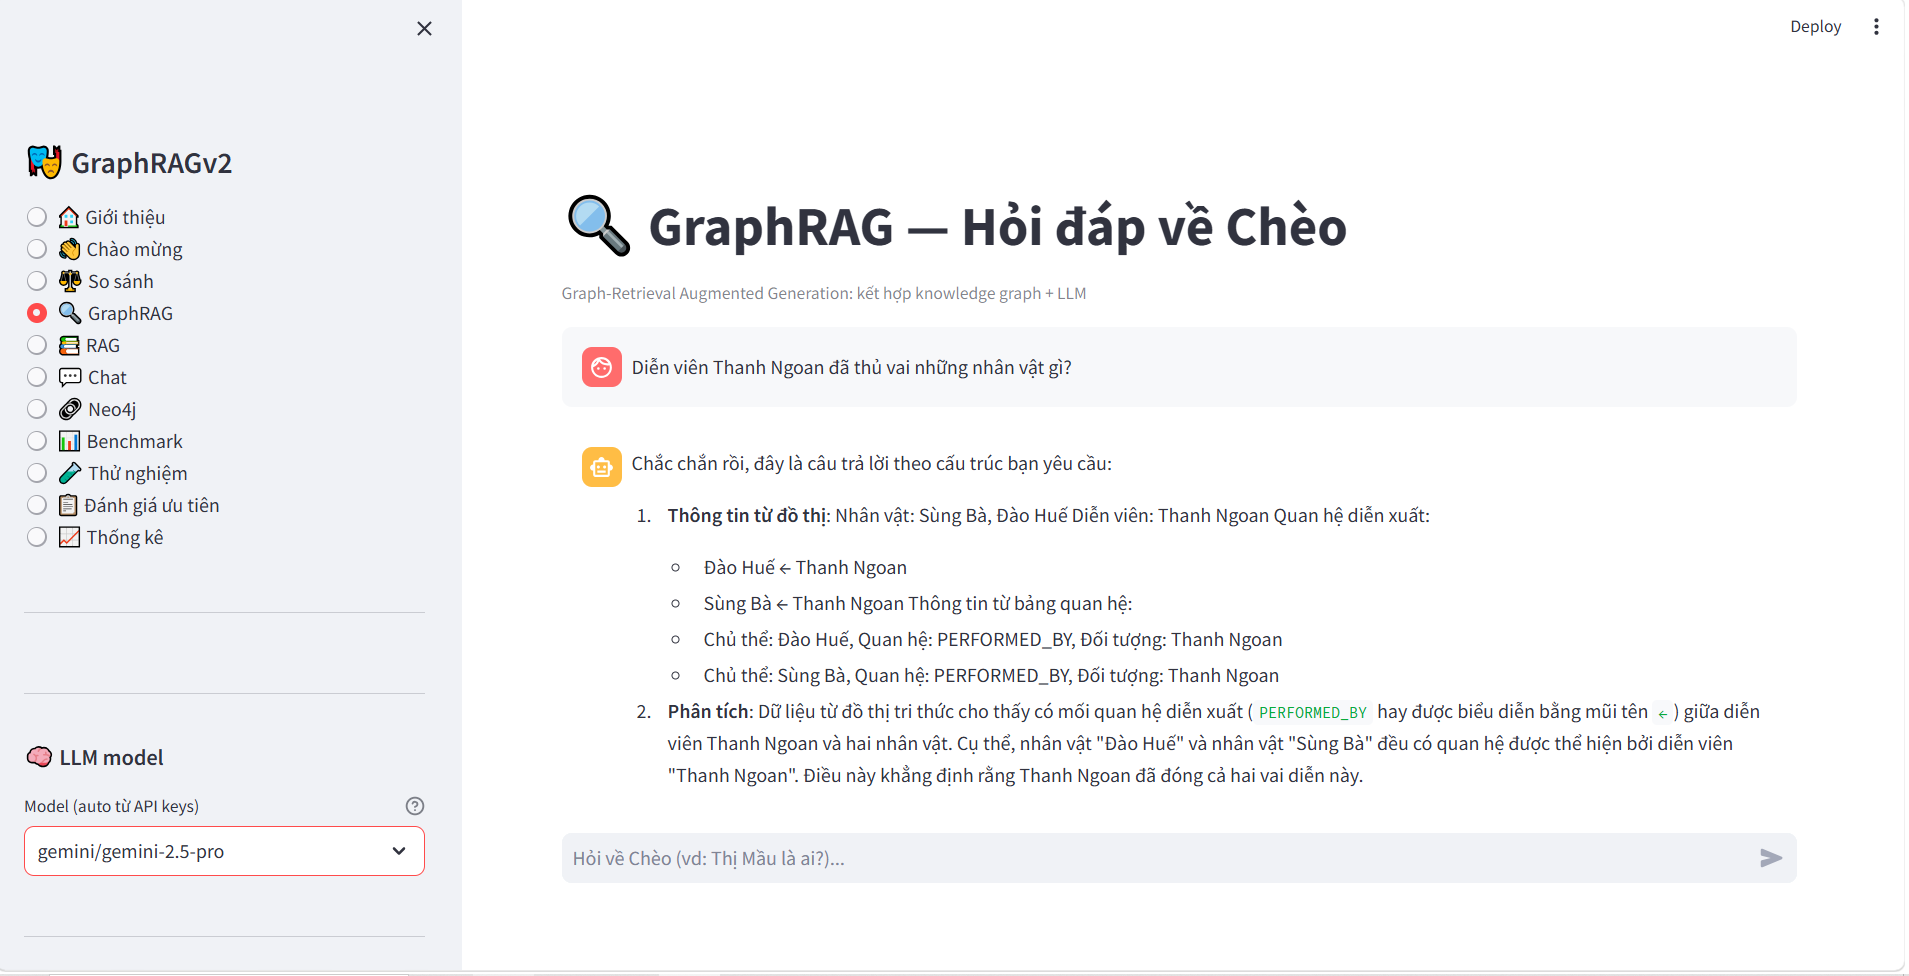
\includegraphics[width=1\linewidth]{figures//c4/UI.png}
    \caption{Giao diện thử nghiệm của hệ thống.}
    \label{fig:UI}
\end{figure}

\subsection{Thiết kế kiểm nghiệm với người dùng}
\label{sec:user_study}

\subsubsection{Chấm điểm đa tiêu chí}
\label{sec:experiment_study}

Hình thức thực nghiệm đầu tiên sử dụng trang Experiment (\textbf{Hình \ref{fig:experiment}}), cho phép người tham gia tự đặt câu hỏi và chấm điểm câu trả lời của ba hệ thống trong thời gian thực. Thử nghiệm tổ chức theo bốn bước: ba bước đầu yêu cầu chọn một câu hỏi trong số bảy câu chuẩn bị sẵn tại mỗi mức độ Dễ, Trung bình và Khó; bước cuối cho phép đặt một câu hỏi tự do. Thiết kế này vừa đảm bảo có câu hỏi có ground truth để so sánh giữa các người tham gia, vừa khảo sát được các câu hỏi tự phát phản ánh nhu cầu thực.

\begin{figure}
    \centering
    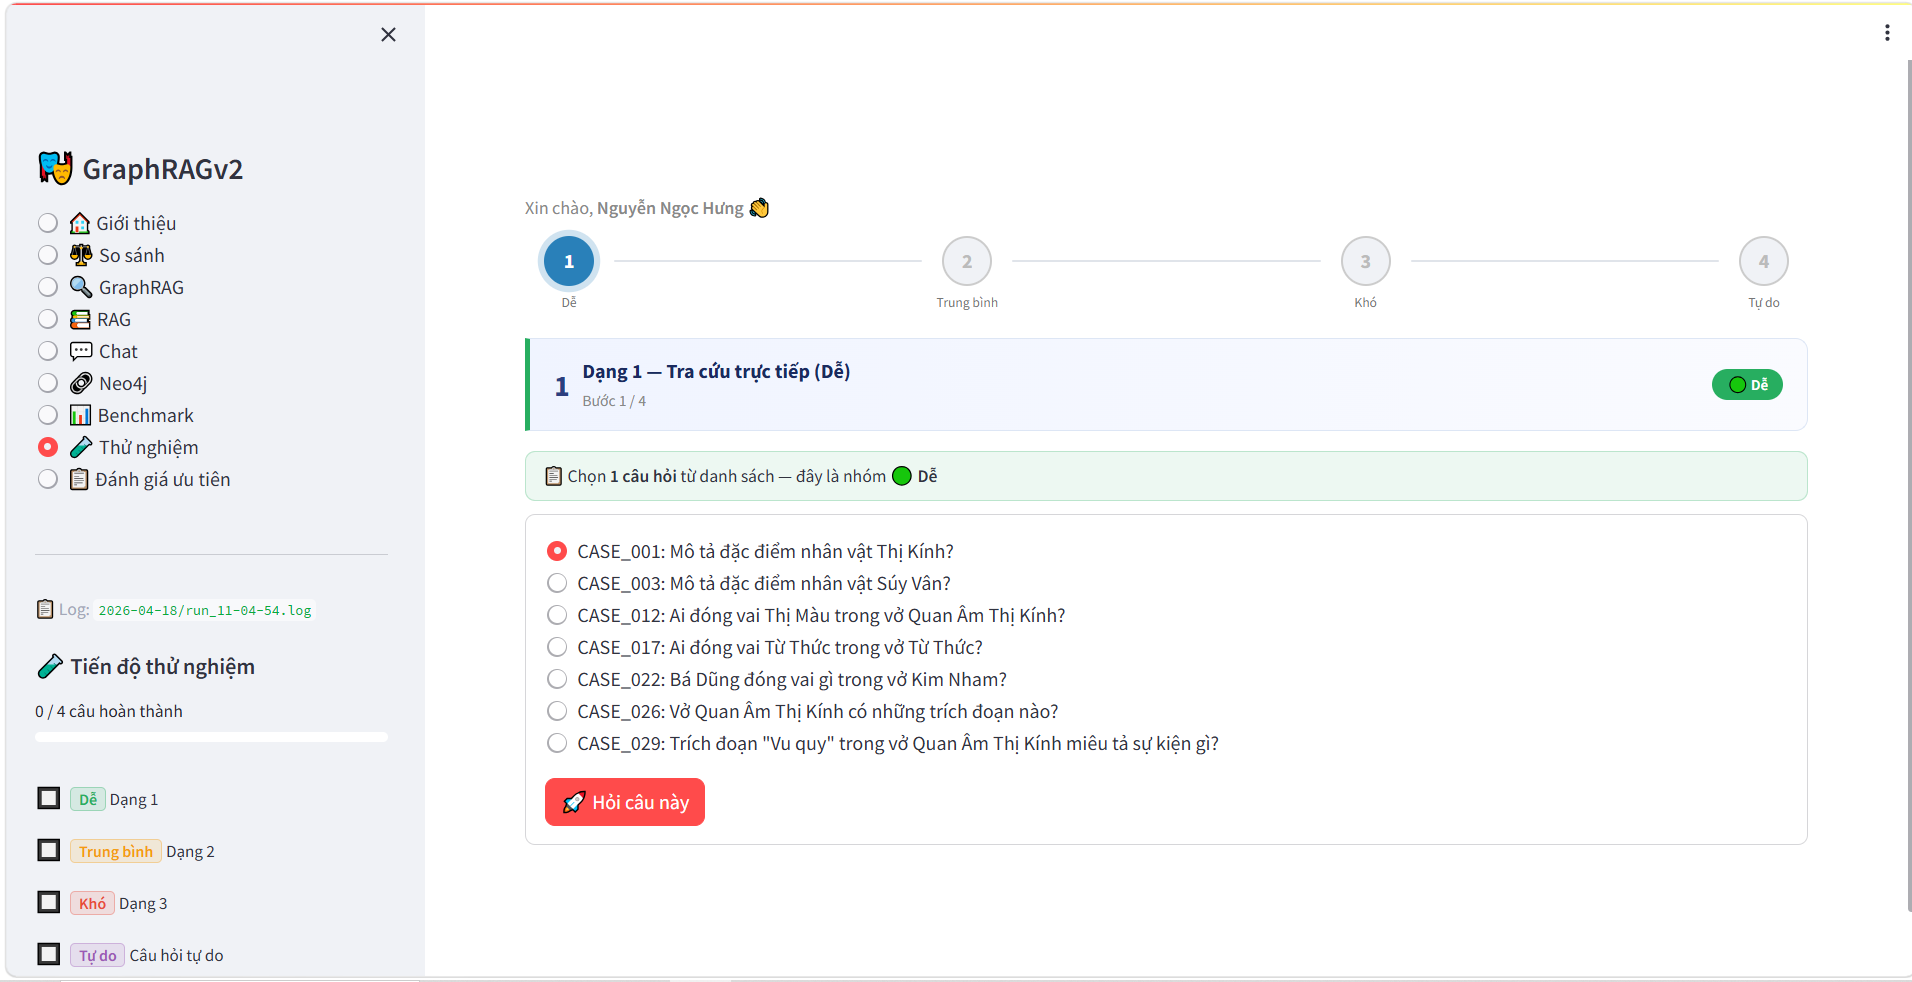
\includegraphics[width=0.9\linewidth]{figures//c4/Experiment.png}
    \caption{Giao diện thực nghiệm hỏi đáp}
    \label{fig:experiment}
\end{figure}

Với mỗi câu, hệ thống chạy đồng thời ba pipeline và hiển thị câu trả lời song song trong ba cột ẩn danh. Người tham gia chấm điểm từng hệ thống theo ba tiêu chí trên thang 1--5: \textit{Chính xác} (thông tin có đúng không), \textit{Đầy đủ} (bao quát nội dung câu hỏi) và \textit{Tự nhiên} (dễ đọc, mạch lạc); đồng thời chọn hệ thống tổng thể tốt nhất. Sau bốn bước, người tham gia trả lời khảo sát hậu nghiệm về mức độ hiểu biết Chèo, tần suất sử dụng công cụ AI, tiêu chí đặt nặng nhất khi lựa chọn và các loại lỗi thường gặp.

Đối tượng tham gia hình thức này là sinh viên, đại diện cho người dùng phổ thông không có kiến thức chuyên sâu về Chèo. Cách chọn đối tượng này nhằm phản ánh trải nghiệm cảm nhận của đông đảo người dùng cuối trong bối cảnh không có điều kiện thẩm định từng chi tiết tri thức. Thông tin hậu nghiệm cho phép phân tích kết quả theo các phân nhóm --- chẳng hạn nhóm có hiểu biết Chèo so với nhóm không có, hoặc nhóm sử dụng AI thường xuyên so với nhóm ít sử dụng.

\subsubsection{Đánh giá so sánh}
\label{sec:preference_study}

Hình thức thực nghiệm thứ hai sử dụng trang Preference (\textbf{Hình \ref{fig:preference}}). Hai mươi mốt câu hỏi tiêu biểu được chọn từ CheoBench v2, bao phủ cả ba nhóm độ khó và nhiều dạng truy vấn từ tra cứu trực tiếp đến phân tích liên vở. Câu trả lời của ba hệ thống đã được sinh sẵn và lưu trữ; người tham gia đọc đồng thời ba câu trả lời hiển thị ẩn danh trong ba cột, chọn câu trả lời tốt nhất và có thể ghi chú nhận xét cho từng câu.

\begin{figure}
    \centering
    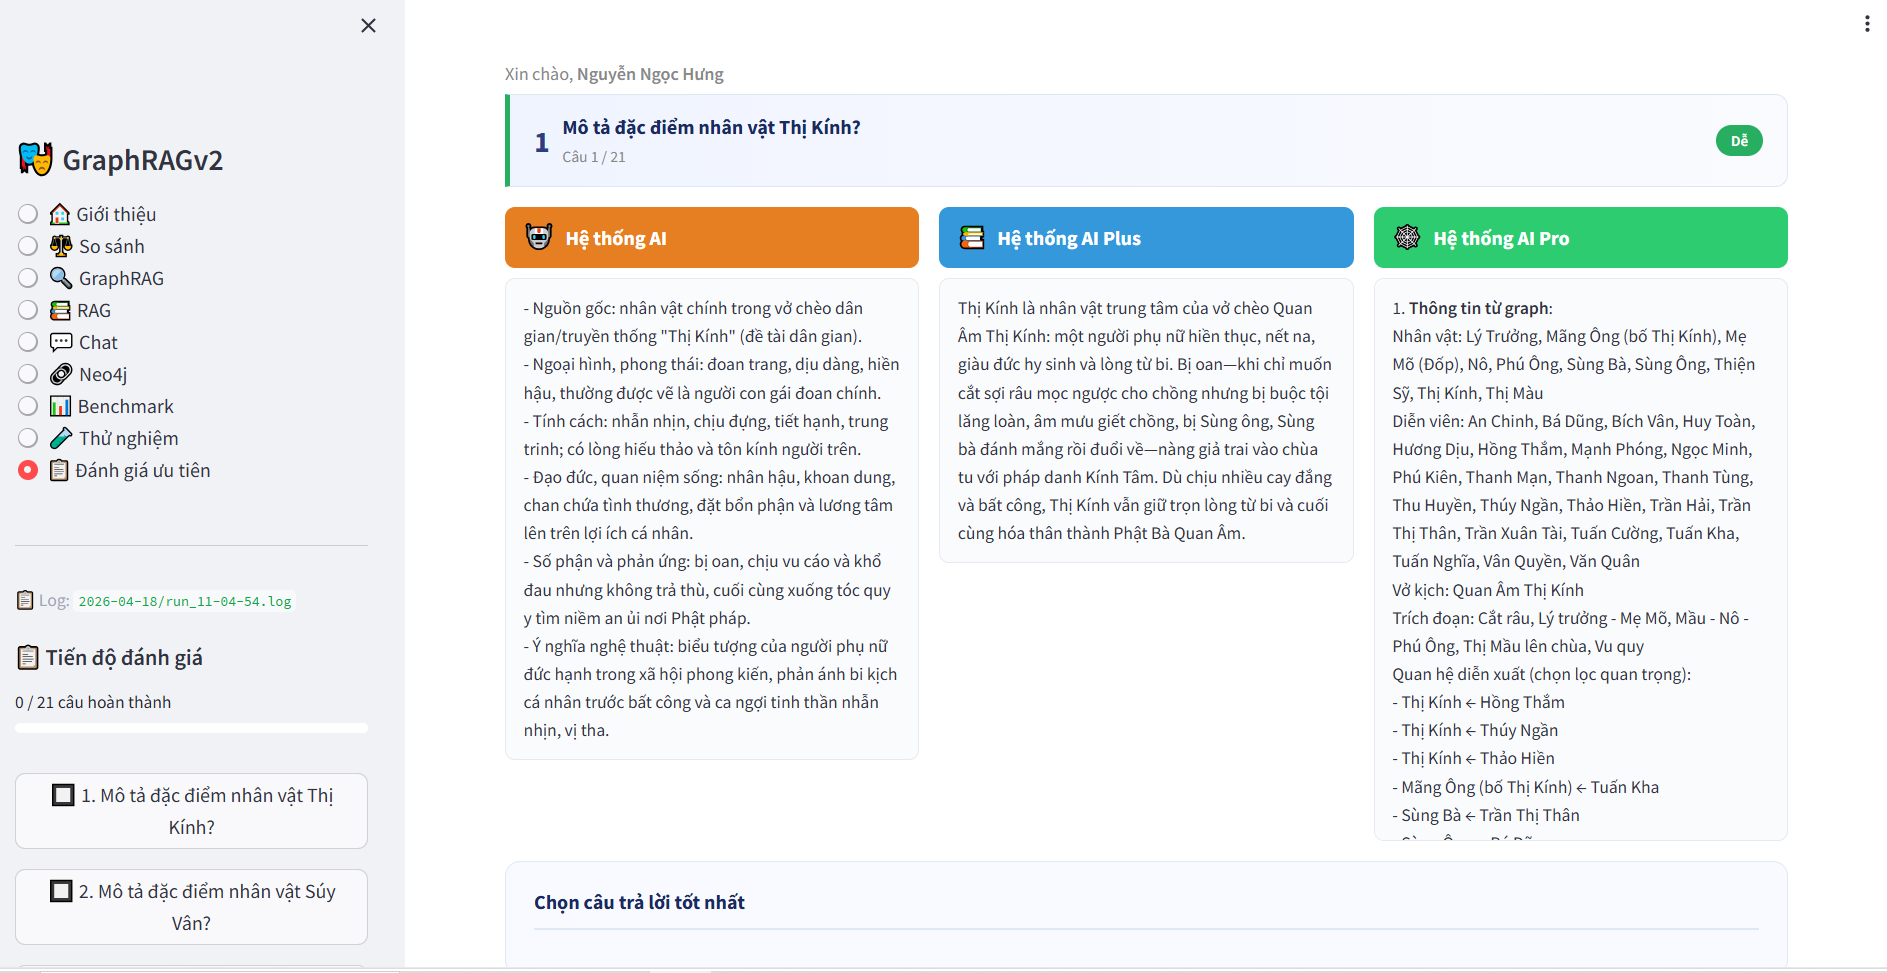
\includegraphics[width=0.9\linewidth]{figures//c4/preference.png}
    \caption{Giao diện thực nghiệm so sánh}
    \label{fig:preference}
\end{figure}

Khác với hình thức trước, Preference không yêu cầu chấm điểm theo thang nhiều mức mà chỉ yêu cầu phán xét tổng thể ``câu trả lời nào là hay nhất''. Định dạng so sánh ba cột trực tiếp giúp người tham gia dễ phát hiện các lỗi tinh tế như chi tiết sai lệch, thiếu sót về nhân vật hoặc mâu thuẫn nội dung --- những lỗi mà các độ đo tự động thường bỏ qua. Việc sử dụng câu trả lời sinh sẵn đảm bảo công bằng: mọi người tham gia đánh giá trên cùng một tập câu trả lời, loại trừ biến động giữa các lần gọi mô hình.

Đối tượng tham gia hình thức này là các chuyên gia có hiểu biết sâu về nghệ thuật Chèo. Kiến thức chuyên môn cho phép họ thẩm định các chi tiết đặc thù của miền --- như tính chính xác của tên nhân vật, mối quan hệ giữa vở diễn, hay sự tinh tế trong cách diễn đạt --- mà người dùng phổ thông khó nắm bắt. Đánh giá của chuyên gia do đó có độ tin cậy cao hơn khi so sánh trực tiếp chất lượng nội dung giữa các hệ thống.

\subsection{Kết quả kiểm nghiệm với người dùng}

\textit{Phần này tổng hợp kết quả của cả hai hình thức kiểm nghiệm. Do quá trình thu thập dữ liệu người dùng vẫn đang tiếp tục tại thời điểm viết báo cáo, các số liệu chi tiết sẽ được bổ sung trong phiên bản hoàn chỉnh.}

% [Placeholder — cập nhật khi có dữ liệu thu thập đầy đủ]
% - Kết quả hình thức 1 (sinh viên): phân bổ phiếu hệ thống tốt nhất, điểm trung bình ba tiêu chí theo từng hệ thống, phân tích theo phân nhóm hiểu biết Chèo.
% - Kết quả hình thức 2 (chuyên gia): phân bổ phiếu chọn, phân tích định tính từ ghi chú.
% - Đối sánh giữa đánh giá sinh viên và đánh giá chuyên gia.
% - Đối sánh giữa đánh giá chủ quan và đánh giá khách quan từ các độ đo ở Mục~\ref{sec:experiments}.

\subsection{Thảo luận trải nghiệm thực tế}

\textit{Phần thảo luận chi tiết sẽ được hoàn thiện khi có đầy đủ dữ liệu kiểm nghiệm người dùng. Dự kiến các điểm thảo luận bao gồm: sự tương đồng và khác biệt giữa đánh giá chủ quan và đánh giá khách quan bằng các độ đo tự động; khác biệt trong cách đánh giá giữa nhóm sinh viên và nhóm chuyên gia; các hạn chế còn lại của hệ thống được bộc lộ qua phản hồi thực tế; và ý nghĩa ứng dụng của hệ thống trong bảo tồn và truyền bá di sản nghệ thuật Chèo.}


\section*{Tiểu kết}
\addcontentsline{toc}{section}{Tiểu kết}

Chương này trình bày quá trình hiện thực hoá và đánh giá hệ thống GraphRAG dựa trên các thiết kế ở Chương 3. Phần cài đặt đã xây dựng môi trường thực nghiệm hoàn chỉnh với Knowledge Graph trên Neo4j, pipeline GraphRAG đầy đủ và hai hệ thống tham chiếu là RAG truyền thống và LLM-only. Ba hệ thống chia sẻ cùng mô hình ngôn ngữ và cùng tham số sinh, đảm bảo chênh lệch kết quả chỉ phản ánh khác biệt về nguồn tri thức và cơ chế truy xuất.

Thực nghiệm định lượng được triển khai với bốn nhóm thí nghiệm tương ứng bốn câu hỏi nghiên cứu, sử dụng hệ thống độ đo đa chiều bao gồm cả chất lượng truy xuất và chất lượng tạo sinh. Kết quả cho thấy kết hợp đa mức độ truy xuất nâng điểm tổng hợp từ 0,54 lên 0,76, định dạng có cấu trúc cho kết quả cao hơn định dạng thiếu quan hệ (0,72 so với 0,65), và Mid-Generation mang lại cân bằng tốt nhất giữa chất lượng và chi phí. So với RAG truyền thống, GraphRAG vượt trội từ +0,10 đến +0,20 điểm trên toàn bộ các độ đo IR, khẳng định lợi ích của cấu trúc đồ thị trong miền tri thức quan hệ phức tạp.

Ở bước triển khai, hệ thống được đưa lên hạ tầng đám mây và kiểm nghiệm với người dùng qua hai hình thức thực nghiệm: chấm điểm đa tiêu chí và đánh giá so sánh. Cách thiết kế này cho phép thu thập phản hồi ở cả mức chi tiết từng tiêu chí lẫn mức phán xét tổng thể, bổ sung cho đánh giá định lượng ở khía cạnh chất lượng chủ quan. Tổng hợp các kết quả trên tạo cơ sở cho những đánh giá tổng kết và hướng phát triển được trình bày trong chương tiếp theo.

